% Template for PLoS
% Version 3.5 March 2018
%
% % % % % % % % % % % % % % % % % % % % % %
%
% -- IMPORTANT NOTE
%
% This template contains comments intended 
% to minimize problems and delays during our production 
% process. Please follow the template instructions
% whenever possible.
%
% % % % % % % % % % % % % % % % % % % % % % % 
%
% Once your paper is accepted for publication, 
% PLEASE REMOVE ALL TRACKED CHANGES in this file 
% and leave only the final text of your manuscript. 
% PLOS recommends the use of latexdiff to track changes during review, as this will help to maintain a clean tex file.
% Visit https://www.ctan.org/pkg/latexdiff?lang=en for info or contact us at latex@plos.org.
%
%
% There are no restrictions on package use within the LaTeX files except that 
% no packages listed in the template may be deleted.
%
% Please do not include colors or graphics in the text.
%
% The manuscript LaTeX source should be contained within a single file (do not use \input, \externaldocument, or similar commands).
%
% % % % % % % % % % % % % % % % % % % % % % %
%
% -- FIGURES AND TABLES
%
% Please include tables/figure captions directly after the paragraph where they are first cited in the text.
%
% DO NOT INCLUDE GRAPHICS IN YOUR MANUSCRIPT
% - Figures should be uploaded separately from your manuscript file. 
% - Figures generated using LaTeX should be extracted and removed from the PDF before submission. 
% - Figures containing multiple panels/subfigures must be combined into one image file before submission.
% For figure citations, please use "Fig" instead of "Figure".
% See http://journals.plos.org/plosone/s/figures for PLOS figure guidelines.
%
% Tables should be cell-based and may not contain:
% - spacing/line breaks within cells to alter layout or alignment
% - do not nest tabular environments (no tabular environments within tabular environments)
% - no graphics or colored text (cell background color/shading OK)
% See http://journals.plos.org/plosone/s/tables for table guidelines.
%
% For tables that exceed the width of the text column, use the adjustwidth environment as illustrated in the example table in text below.
%
% % % % % % % % % % % % % % % % % % % % % % % %
%
% -- EQUATIONS, MATH SYMBOLS, SUBSCRIPTS, AND SUPERSCRIPTS
%
% IMPORTANT
% Below are a few tips to help format your equations and other special characters according to our specifications. For more tips to help reduce the possibility of formatting errors during conversion, please see our LaTeX guidelines at http://journals.plos.org/plosone/s/latex
%
% For inline equations, please be sure to include all portions of an equation in the math environment.  For example, x$^2$ is incorrect; this should be formatted as $x^2$ (or $\mathrm{x}^2$ if the romanized font is desired).
%
% Do not include text that is not math in the math environment. For example, CO2 should be written as CO\textsubscript{2} instead of CO$_2$.
%
% Please add line breaks to long display equations when possible in order to fit size of the column. 
%
% For inline equations, please do not include punctuation (commas, etc) within the math environment unless this is part of the equation.
%
% When adding superscript or subscripts outside of brackets/braces, please group using {}.  For example, change "[U(D,E,\gamma)]^2" to "{[U(D,E,\gamma)]}^2". 
%
% Do not use \cal for caligraphic font.  Instead, use \mathcal{}
%
% % % % % % % % % % % % % % % % % % % % % % % % 
%
% Please contact latex@plos.org with any questions.
%
% % % % % % % % % % % % % % % % % % % % % % % %

\documentclass[10pt,letterpaper,table]{article}
\usepackage[top=0.85in,left=2.75in,footskip=0.75in]{geometry}

%\usepackage{natbib} % bibliography

\usepackage{setspace}
\usepackage{pgf}
\usepackage{tikz}
\usepackage{bm}
\usetikzlibrary{bayesnet}

\usepackage{tcolorbox} % for text box

\newtcolorbox[auto counter]{mybox}[2][]{width=\textwidth, colback=gray!10, boxrule=0pt, title=Box~\thetcbcounter: #2, #1}


\usepackage{alltt}

% amsmath and amssymb packages, useful for mathematical formulas and symbols
\usepackage{amsmath,amssymb}

% Use adjustwidth environment to exceed column width (see example table in text)
\usepackage{changepage}

% Use Unicode characters when possible
\usepackage[utf8x]{inputenc}

% textcomp package and marvosym package for additional characters
\usepackage{textcomp,marvosym}

% cite package, to clean up citations in the main text. Do not remove.
\usepackage{cite}

% Use nameref to cite supporting information files (see Supporting Information section for more info)
\usepackage{nameref,hyperref}

% line numbers
\usepackage[right]{lineno}

% ligatures disabled
\usepackage{microtype}
\DisableLigatures[f]{encoding = *, family = * }

% color can be used to apply background shading to table cells only
\usepackage{xcolor}

% array package and thick rules for tables
\usepackage{array}

% underline
\usepackage{soul}

% create "+" rule type for thick vertical lines
\newcolumntype{+}{!{\vrule width 2pt}}

% create \thickcline for thick horizontal lines of variable length
\newlength\savedwidth
\newcommand\thickcline[1]{%
  \noalign{\global\savedwidth\arrayrulewidth\global\arrayrulewidth 2pt}%
  \cline{#1}%
  \noalign{\vskip\arrayrulewidth}%
  \noalign{\global\arrayrulewidth\savedwidth}%
}

% \thickhline command for thick horizontal lines that span the table
\newcommand\thickhline{\noalign{\global\savedwidth\arrayrulewidth\global\arrayrulewidth 2pt}%
\hline
\noalign{\global\arrayrulewidth\savedwidth}}


% Remove comment for double spacing
%\usepackage{setspace} 
%\doublespacing

% Text layout
\raggedright
\setlength{\parindent}{0.5cm}
\textwidth 5.25in 
\textheight 8.75in

% Bold the 'Figure #' in the caption and separate it from the title/caption with a period
% Captions will be left justified
\usepackage[aboveskip=1pt,labelfont=bf,labelsep=period,justification=raggedright,singlelinecheck=off]{caption}
\renewcommand{\figurename}{Fig}

% Use the PLoS provided BiBTeX style
\bibliographystyle{plos2015}

% Remove brackets from numbering in List of References
\makeatletter
\renewcommand{\@biblabel}[1]{\quad#1.}
\makeatother



% Header and Footer with logo
\usepackage{lastpage,fancyhdr,graphicx}
\usepackage{epstopdf}
%\pagestyle{myheadings}
\pagestyle{fancy}
\fancyhf{}
%\setlength{\headheight}{27.023pt}
%\lhead{\includegraphics[width=2.0in]{PLOS-submission.eps}}
\rfoot{\thepage/\pageref{LastPage}}
\renewcommand{\headrulewidth}{0pt}
\renewcommand{\footrule}{\hrule height 2pt \vspace{2mm}}
\fancyheadoffset[L]{2.25in}
\fancyfootoffset[L]{2.25in}
\lfoot{\today}

%% Include all macros below

\newcommand{\lorem}{{\bf LOREM}}
\newcommand{\ipsum}{{\bf IPSUM}}

% next 6 lines put a caption on \alltt float
\usepackage{newfloat}
\usepackage{caption}
\DeclareFloatingEnvironment[fileext=frm,placement={!ht},name=example]{example}
\DeclareCaptionSubType*{example}
% \captionsetup[subexample]{name=Example}
% \renewcommand{\thesubexample}{\theexample}

\usepackage{listing}

%% END MACROS SECTION


\begin{document}
\vspace*{0.2in}

% Title must be 250 characters or less.
\begin{flushleft}
{\Large
\textbf\newline{LinguaPhylo: a probabilistic model specification language for
  reproducible phylogenetic analyses} % Please use "sentence case" for title and headings (capitalize only the first word in a title (or heading), the first word in a subtitle (or subheading), and any proper nouns).
}
\newline
% Insert author names, affiliations and corresponding author email (do not include titles, positions, or degrees).
\\
Alexei J. Drummond\textsuperscript{1,2,3}*,
Dong Xie\textsuperscript{1,3},
F\'{a}bio K Mendes\textsuperscript{1,2}
\\
\bigskip
\textbf{1} Centre for Computational Evolution, University of Auckland, Auckland, New Zealand
\\
\textbf{2} School of Biological Sciences, University of Auckland, Auckland, New Zealand
\\
\textbf{3} School of Computer Science, University of Auckland, Auckland, New Zealand
\\
\bigskip

% Insert additional author notes using the symbols described below. Insert symbol callouts after author names as necessary.
% 
% Remove or comment out the author notes below if they aren't used.
%
% Primary Equal Contribution Note

% Use the asterisk to denote corresponding authorship and provide email address in note below.
* a.drummond@auckland.ac.nz

\end{flushleft}
% Please keep the abstract below 300 words
\section*{Abstract}
  Phylogenetic models have become increasingly complex and the data sets addressed larger and more rich.
  Yet there is no succinct language to accurately specify the details of a phylogenetic model for the purposes of reproducibility or reuse.
  We present a new language to specify the details of a phylogenetic model that is both human and machine readable.
  We also report on the development of a graphical software package that can be used to construct and simulate data from
  models in this new language, as well as create natural language narratives that can form the basis of a description of the model for the method section of a manuscript.
  Finally we report on a command-line program that can be used to generate XML for the BEAST2 software package based
  on a model specified in this new language.
  These tools together should aid in the goal of reproducibility and reuse of probabilistic phylogenetic models.


% Please keep the Author Summary between 150 and 200 words
% Use first person. PLOS ONE authors please skip this step. 
% Author Summary not valid for PLOS ONE submissions.   
\section*{Author summary}
  We describe a succinct domain-specific language to accurately specify the details of a phylogenetic model for the purposes of reproducibility or reuse.
  In addition we have developed a graphical software package that can be used to construct and simulate data from models described in this new language, as well as create natural language narratives that can form the basis of a description of the model for the method section of a manuscript.
  Finally we report on a command-line program that can be used to generate XML for the BEAST2 software package based on a model specified in this new language.
  These tools together should aid in the goal of reproducibility and reuse of probabilistic phylogenetic models. 


\linenumbers

% Use "Eq" instead of "Equation" for equation citations.
\section*{Introduction}

Transparency is a scientific ideal, and replicability and
reproducibility lie at the heart of the scientific endeavor
\cite{nas19,munafo17}. 
Metaresearch efforts have uncovered the so-called ``reproducibility
crisis'' \cite{baker16} in many scientific domains \cite{baker16}. 
In recent years, the growing number of computational biology software available enables greater freedom in data analyses, 
but at the cost of increased complexity in the data-preparation and analytical pipelines \cite{eren2021community}. 
This increases the difficulty of accurately reporting, re-executing and re-using analyses. 
These barriers have been recognized by the wider genomics research community \cite{eren2021community} as well as within evolutionary biology \cite{oakley2014osiris}. 

In evolutionary biology, phylogenetics has become a highly technical discipline \cite{oakley2014osiris}. 
The most general phylogenetic tools are Bayesian methods (e.g., BEAST, BEAST 2, MrBayes and
RevBayes; \cite{beast,beast2,revbayes,mrbayes}) 
that can simultaneously reconstruct phylogenetic tree topology and divergence times, as well as estimate the related micro-evolutionary and macro-evolutionary parameters. 
Phylogenetic analyses often combine 
multiple models within a complex pipeline to answer questions in evolutionary biology such as species evolution \cite{gavryushkina17,ogilvie21,zhang21}, ancestral bio-geographical ranges \cite{lemey10,landis18}, and 
% ecological networks \cite{braga20}, 
% trait evolution \cite{may19,bite}, and 
epidemics \cite{faria21,douglas21}. 
Reproducing and reusing a phylogenetics pipeline is no easy task. 
Often requiring the user to understand the input data format, the evolutionary models, details of the model parameters, as well as software runtime parameters. 
Runtime parameters can include Markov chain Monte Carlo (MCMC) sampling parameters which are not inherently part of the model.
Currently, little research has been done on the readability and re-usability of phylogenetic models. 
Our paper presents a tool aimed to: (i) facilitate accurate communication of phylogenetic analyses, (ii) improve reproducibility, and (iii) increase re-usability of phylogenetic analyses on new datasets. 
 
Previous attempts to address model specification and analysis setup include BEAST style XMLs (eXtensible Markup Language) developed for BEAST software \cite{beast,beast2} and the Rev language for RevBayes \cite{revbayes}. 
The extensibility of XMLs provides flexibility to developers allowing them to create new
descriptive tags for specifying new models.
However, BEAST style XMLs are difficult for humans to read and interpret due to the verbose syntax and interconnected components that make up BEAST models. 
This also makes it difficulty to translate BEAST or BEAST2 analyses from text descriptions in published work. 
On the other hand, the Rev language 
\cite{revbayes} 
incorporates conventional notation from probability theory. 
This feature makes Rev model specification more intuitive, but still requires users to contend with runtime 
details %extraneous to the model 
such as MCMC parameters and the operator schedule.

Here, we introduce LinguaPhylo (LPhy), an open-source programming
language focused on model specification to improve reproducibility, re-usability and model readability. 
\textcolor{blue}{[Highlights of LPhy should go here...]}
Our software includes a graphical user interface as well as a command line interface. 
Additionally, we introduce a tool, LPhyBEAST, for integrating model specification with phylogenetic analysis via BEAST2.
The software presented in this paper aims to make it easier to report,
validate and simulate complex phylogenetic models, as well as to reproduce and re-use phylogenetic analyses.

\section*{Design and Implementation}

% \subsection*{A concise domain-specific language for phylogenetic inference}
The LPhy language is designed to enable the specification of probabilistic phylogenetic models using a concise and readible syntax. 
It is built on top of Java and provides the following features: 
(i) data simulation from phylogenetic generative distributions, (ii) R-style vectorization of parameters, (iii) extensibility mechanism for new functions and data types, (iv) integration with phylogenetic inference software such as BEAST2, and (v) easy dataset swapping for re-use of phylogenetic models on new datasets.

Example \ref{lphy:rsva} shows an LPhy script for performing phylogenetic inference on a virus dataset containing sequences of the Respiratory syncytial virus subgroup A (RSVA). 
This script concisely specifies a phylogenetic analysis using 19 lines of code.  
The code contains a \textbf{data block} for specifying the input dataset, and a \textbf{model block} which defines the phylogenetic model. 
% An accompanying tutorial for this analysis is publicly available at \url{www.linguaphylo.gihub.io/tutorials/time-stamped-data/}.
% We have modified the script slightly for illustrative purposes:

{
  \small
  \begin{listing}
    \stepcounter{example}
    \begin{alltt}
      data \{
      options = \{\textcolor{gray}{ageDirection=}\textcolor{magenta}{"forward"}, \textcolor{gray}{ageRegex=}\textcolor{magenta}{"s(\textbackslash{}d+)"}\};
      nexusFilePath = \textcolor{magenta}{"tutorials/data/RSV2.nex"};
      D = \textcolor{magenta!80!black}{readNexus}(\textcolor{gray}{file=}nexusFilePath, \textcolor{gray}{options=}options);
      codon = D.\textcolor{magenta!80!black}{charset}([\textcolor{magenta}{"3-629\textbackslash{}3"}, \textcolor{magenta}{"1-629\textbackslash{}3"}, \textcolor{magenta}{"2-629\textbackslash{}3"}]);
      n = 3;
      L = [209, 210, 210];
      taxa = D.\textcolor{magenta!80!black}{taxa}();
      \}
      model \{
      \textcolor{green}{\(\pi\)} \textasciitilde \textcolor{blue}{Dirichlet}(\textcolor{gray}{replicates=}n, \textcolor{gray}{conc=}[\textcolor{magenta}{2.0}, \textcolor{magenta}{2.0}, \textcolor{magenta}{2.0}, \textcolor{magenta}{2.0}]);
      \textcolor{green}{\(\kappa\)} ~ \textcolor{blue}{LogNormal}(\textcolor{gray}{sdlog=}\textcolor{magenta}{0.5}, \textcolor{gray}{meanlog=}\textcolor{magenta}{1.0}, \textcolor{gray}{replicates=}n);
      \textcolor{green}{r} ~ \textcolor{blue}{WeightedDirichlet}(\textcolor{gray}{conc=}\textcolor{magenta!80!black}{rep}(\textcolor{gray}{element=}\textcolor{magenta}{1.0}, \textcolor{gray}{times=}n), \textcolor{gray}{weights=}L);
      \textcolor{green}{\(\mu\)} ~ \textcolor{blue}{LogNormal}(\textcolor{gray}{meanlog=}\textcolor{magenta}{-5.0}, \textcolor{gray}{sdlog=}\textcolor{magenta}{1.25});
      \textcolor{green}{\(\Theta\)} ~ \textcolor{blue}{LogNormal}(\textcolor{gray}{meanlog=}\textcolor{magenta}{3.0}, \textcolor{gray}{sdlog=}\textcolor{magenta}{2.0});
      \textcolor{green}{\(\psi\)} ~ \textcolor{blue}{Coalescent}(\textcolor{gray}{taxa=}taxa, \textcolor{gray}{theta=}\textcolor{green}{\(\Theta\)});
      Q = \textcolor{magenta!80!black}{hky}(\textcolor{gray}{kappa=}\textcolor{green}{\(\kappa\)}, \textcolor{gray}{freq=}\textcolor{green}{\(\pi\)}, \textcolor{gray}{meanRate=}\textcolor{green}{r});
      \textcolor{green}{codon} ~ \textcolor{blue}{PhyloCTMC}(\textcolor{gray}{L=}L, \textcolor{gray}{Q=}Q, \textcolor{gray}{mu=}\textcolor{green}{\(\mu\)}, \textcolor{gray}{tree=}\textcolor{green}{\(\psi\)});
      \}
    \end{alltt}
    % \captionof{subexample}{LPhy script specifying a phylodynamic model
    \caption{An LPhy script for phylodynamic analysis of a virus dataset containing Respiratory syncytial virus subgroup A (RSVA) genomic samples.
    \newline}
    \label{lphy:rsva}
  \end{listing}
}

% Briefly, the script above (Example \ref{lphy:rsva}) specifies a
% phylodynamic model to be used with molecular sequences from the
% Respiratory syncytial virus subgroup A (RSVA).
% Commands related to parsing input data and to specifying the model are
% enclosed within the `\texttt{data \{ \}}' and `\texttt{model \{ \}}'
% blocks, respectively.
% We will explain what each line accomplishes in the following sections.


% \begin{mybox}[label=box1, float=htpb!]{A simple phylogenetic model}
%  % \begin{minipage}[t]{0.60\textwidth}
 
%  \begin{enumerate}
%  \item Modeling language
%     {\singlespacing
% \begin{alltt}
% model \{
%   \textcolor{green}{\(\lambda\)} ~ \textcolor{blue}{LogNormal}(\textcolor{gray}{meanlog=}\textcolor{magenta}{3.0}, \textcolor{gray}{sdlog=}\textcolor{magenta}{1.0});
%   \textcolor{green}{\(\psi\)} ~ \textcolor{blue}{Yule}(\textcolor{gray}{lambda=}\textcolor{green}{\(\lambda\)}, \textcolor{gray}{n=}\textcolor{magenta}{16});
%   \textcolor{green}{D} ~ \textcolor{blue}{PhyloCTMC}(\textcolor{gray}{L=}\textcolor{magenta}{200}, \textcolor{gray}{Q=}\textcolor{magenta!80!black}{jukesCantor}(), \textcolor{gray}{tree=}\textcolor{green}{\(\psi\)});
% \}
% \end{alltt}
% }
% %  \end{minipage}%
% %\begin{minipage}[t]{0.40\textwidth}
% \item Graphical model
% \\\\
% {\centering
% \begin{tikzpicture}[scale=0.52,
% dstyle/.style={draw=blue!50,fill=blue!20},
% vstyle/.style={draw=green,fill=green!20},
% cstyle/.style={font=\small},
% detstyle/.style={draw=red!50,fill=red!20}
% ]
% \node[const, cstyle] at (1.0, -0.0) (602717583) {meanlog = 3.0};
% \node[const, cstyle] at (5.0, -0.0) (897996787) {sdlog = 1.0};
% \node[latent, vstyle] at (2.0, -4.0) (lambda) {$\lambda$};
% \node[const, cstyle] at (6.0, -4.0) (2011155364) {n = 16};
% \node[latent, vstyle] at (2.0, -8.0) (psi) {$\psi$};
% \node[const, cstyle] at (6.0, -8.0) (1992433642) {L = 200};
% \node[det, detstyle] at (10.0, -8.0) (258223775) {[Q]};
% \node[latent, vstyle] at (6.0, -12.0) (D) {D};
% \factor[above=of lambda] {LogNormallambda} {left:LogNormal} {} {} ; %
% \factoredge {602717583, 897996787} {LogNormallambda} {lambda}; %
% \factor[above=of psi] {Yulepsi} {left:Yule} {} {} ; %
% \factoredge {lambda, 2011155364} {Yulepsi} {psi}; %
% \factor[above=of 258223775] {jukesCantor258223775} {left:jukesCantor} {} {} ; %
% \factoredge {} {jukesCantor258223775} {258223775}; %
% \factor[above=of D] {PhyloCTMCD} {left:PhyloCTMC} {} {} ; %
% \factoredge {1992433642, 258223775, psi} {PhyloCTMCD} {D}; %
% \end{tikzpicture}}
% %\end{minipage}

% \item Posterior

% $$P(\psi, \lambda | D) \propto P(D | \psi) P(\psi | \lambda) P(\lambda) $$

% \end{enumerate}

% \end{mybox}

% Each of the lines in this model specification expresses how a random
% variable (to the left of the tilde) is generated by a generative
% distribution to the right.

% The first line creates a random variable (\texttt{lambda}), that is
% log-normally distributed.
% The second line creates a tree (\texttt{tree}) with 16 taxa from the
% Yule process with a lineage birth rate equal to \texttt{lambda}.
% The third line produces a multiple sequence alignment (\texttt{D})
% with a length of 200, by simulating a Jukes Cantor model of sequence
% evolution down the branches of  \texttt{tree}.
% As you can see, each of the random variables depends on the previous,
% so this is a hierarchical model that ultimately defines a probability
% distribution over sequence alignments of size $16 \times 200$.

% To construct an analysis of a data set with this model we add a data block:

% {\small
% \begin{alltt}
% data \{
%   D = \textcolor{magenta!80!black}{readNexus}(\textcolor{gray}{file=}\textcolor{magenta}{"data/primate.nex"});
%   L = D.\textcolor{magenta!80!black}{nchar}();
%   taxa = D.\textcolor{magenta!80!black}{taxa}();
% \}
% model \{
%   \textcolor{green}{lambda} ~ \textcolor{blue}{LogNormal}(\textcolor{gray}{meanlog=}\textcolor{magenta}{3.0}, \textcolor{gray}{sdlog=}\textcolor{magenta}{1.0});
%   \textcolor{green}{tree} ~ \textcolor{blue}{Yule}(\textcolor{gray}{lambda=}\textcolor{green}{lambda}, \textcolor{gray}{taxa=}taxa);
%   \textcolor{green}{D} ~ \textcolor{blue}{PhyloCTMC}(\textcolor{gray}{L=}L, \textcolor{gray}{Q=}\textcolor{magenta!80!black}{jukesCantor}(), \textcolor{gray}{tree=}\textcolor{green}{tree});
% \}
% \end{alltt}}

% These two blocks of statements contain all the information needed to define
% a Bayesian phylogenetic analysis of a multiple sequence alignment.
% The data block may contain literals, and deterministic values, including those read in from a file, but not random variables or generative distributions.
% The model block contains all random variables, generative distributions and boundary conditions that define the model.
% If a value in the data block has the same name as a random variable in the model block, then that signifies that the data block value is an observation of the random variable with the same name.


% So by assigning the alignment in file
% ``data/primate.nex'' to the name D in the data block we are saying that the random variable in the model named D has
% been observed, and we will infer all the other random variables
% (tree and lambda in this example) in the model from that observed sequence alignment.

\subsection*{Language features}
Similar to other programming languages, LPhy allows variables to be declared as primitives, objects or arrays.
In addition to this, the LPhy language provides features specific to phylogenetic models including: probabilistic distributions (e.g., Normal and Exponential distributions), tree generative distributions such as birth-death and coalescent processes, sequence generators such as substitution models (e.g., the general-time-reversible model \cite{gtr}), tree data and sequence alignment data. 
Our software natively supports input sequences in nexus and fasta formats and trees in newick format. 
Table \ref{tab:generators} shows the range of phylogentic specific methods currently implemented within the LPhy language.

\begin{table}[h]
  \caption{A list of methods supported by
    the LinguaPhylo language.}
  \begin{tabular}{|l|l|l|}
    \hline
    Method type & Example & Reference \\\hline
    Probabilistic distributions & \texttt{Uniform()} &\\
              & \texttt{Normal()} &\\
              & \texttt{LogNormal()} &\\
              & \texttt{Exponential()} &\\
              & \texttt{Gamma()} &\\
              & \texttt{Dirichlet()} &\\ \hline
    Tree generators & \texttt{Yule()} & \cite{yule1925ii}\\
              & \texttt{BirthDeath()} &\\
              & \texttt{FullBirthDeath()} &\\
              & \texttt{BirthDeathSampling()} &\\
              & \texttt{BirthDeathSerialSampling()} & \cite{stadler2013dating}\\
              & \texttt{Coalescent()} & \cite{kingman82}\\
              & \texttt{SkylineCoalescent()} & \cite{pybus00,drummond2005bayesiansequences}\\
              & \texttt{StructuredCoalescent()} &\\
              & \texttt{MultispeciesCoalescent()} &\\\hline
    Sequence generators & \texttt{jukesCantor()} & \cite{jc69}\\
              & \texttt{hky()} & \cite{hky}\\
              & \texttt{gtr()} & \cite{gtr}\\ \hline
    Input parsers & \texttt{newick()} &\\
              & \texttt{readNexus()} &\\\hline
    Other methods & \texttt{length()} &\\
    & \texttt{nchar()} &\\
    & \texttt{taxa()} &\\ \hline
  \end{tabular}
  \label{tab:generators}
\end{table}

% \subsubsection*{Values}
% Values in LinguaPhylo represent either atomic or arrays of random
% variables or constants, which can be of standard
% primitive types (e.g., \texttt{Boolean}, \texttt{Integer},
% \texttt{Double}, \texttt{String}) or more complex types (e.g.,
% \texttt{Alignment}, \texttt{TimeTree}).
% The type system of LPhy is not limited to aforementioned types,
% however, and new types can be added to its Java implementation.\newline 

% % \begin{table}[h]
% %   \begin{tabular}{lllll}
% %     \hline
% %     Value & Form & Type & Example\\\hline
% %     Constant & Atomic & Primitive & \texttt{Integer}, \texttt{Double},
% %                                     \texttt{String}, \texttt{Boolean}\\
% %           & & Object & \texttt{Alignment}, \texttt{TimeTree}\\
% %           & Array & Primitive & (Array form of its atomic counterpart)\\
% %           & & Object & (Array form of its atomic counterpart)\\\hline
% %     Random variable & Atomic & Primitive\\
% %           & & Object\\
% %           & Array & Primitive\\
% %           & & Object\\ 
% % \end{tabular}
% % \end{table}

% \noindent \emph{Atomic primitive constants}. The simplest type of
% values in LinguaPhylo is an atomic primitive constant.
% In the lines below (extracted from Example \ref{lphy:rsva}), we define
% two primitive constants: a \texttt{String} constant named
% \texttt{nexusFilePath}, and a \texttt{Integer} constant named
% \texttt{n}:

% {
% \small
% \begin{alltt}
%   nexusFilePath = \textcolor{magenta}{"tutorials/data/RSV2.nex"};
%   n = 3;
% \end{alltt}
% }

% In LPhy there is no explicit statement of types, which are
% automatically inferred.
% \texttt{nexusFilePath} is inferred to be a \texttt{String} because its
% literal value is surrounded by double quotes.
% Constant \texttt{n} is inferred to be an \texttt{Integer} because
% string `\texttt{3}' string has no decimal point or fractional component
% (conversely, \texttt{Double} would be inferred if 
% the string had a fractional component).\newline

% % The first line defines a constant named `a' with a value of
% % `2.0'. There is no explicit statement of the type, which is simply
% % inferred to be a Double because the literal string `2.0' has a
% % fractional component. The second constant `b' here is a constant of
% % type Integer because it has no decimal point or fractional
% % component. The third constant is of primitive type Boolean, inferred
% % by the keyword `true'. the last constant is of type String because of
% % the double quotes surrounding the literal value.


% % {\singlespacing
% % \begin{alltt}
% %   a = 2.0;
% %   b = 2;
% %   c = true;
% %   d = "lphy";
% % \end{alltt}
% % }

% \noindent \emph{Arrays of primitive constants}. The notion of primitives
% can be extended to arrays.
% In order to declare a constant array, comma-delimited literals should
% be enclosed in square brackets as shown below:

% {\small
%   \begin{alltt}
%     L = [209, 210, 210];
%   \end{alltt}  
% }

% For sequences of consecutive integers, a more compact notation can be
% employed using the `\texttt{:}' character to define a range.
% In the example below, constant arrays \texttt{a} and \texttt{b}
% represent the same sequence of consecutive integers from 1 to 10
% inclusive.

% \begin{alltt}
%   a = [1, 2, 3, 4, 5, 6, 7, 8, 9, 10];
%   b = 1:10;
% \end{alltt}

\subsubsection*{Probabilistic distributions}
...

{\singlespacing
\begin{alltt}
  \textcolor{green}{\(\mu\)} ~ \textcolor{blue}{LogNormal}(\textcolor{gray}{meanlog=}\textcolor{magenta}{-5.0}, \textcolor{gray}{sdlog=}\textcolor{magenta}{1.25});
  \textcolor{green}{\(\Theta\)} ~ \textcolor{blue}{LogNormal}(\textcolor{gray}{meanlog=}\textcolor{magenta}{3.0}, \textcolor{gray}{sdlog=}\textcolor{magenta}{2.0});
\end{alltt}
}


\subsubsection*{Tree generators}
...

{\small
  \begin{alltt}
    \textcolor{green}{\(\psi\)} ~ \textcolor{blue}{Coalescent}(\textcolor{gray}{taxa=}taxa, \textcolor{gray}{theta=}\textcolor{green}{\(\Theta\)});
  \end{alltt}
}

\subsubsection*{Sequence generators}
...

\subsubsection*{Generators}
% As their name suggests, generators generate atomic or arrays of
% values.
% Generators can be generative distributions, deterministic functions,
% or method calls (Table \ref{tab:lphygenerators}).
Like values, new generators can also be added to LPhy's Java
implementation (see Results section below).\newline

\noindent \emph{Generative distributions}. A generative distribution
generates a named random variable value, which can have an object or a
primitive type.
Some generative distributions have labelled parameters, like the
following lines from the full script in the previous section:

{\singlespacing
\begin{alltt}
  \textcolor{green}{\(\mu\)} ~ \textcolor{blue}{LogNormal}(\textcolor{gray}{meanlog=}\textcolor{magenta}{-5.0}, \textcolor{gray}{sdlog=}\textcolor{magenta}{1.25});
  \textcolor{green}{\(\Theta\)} ~ \textcolor{blue}{LogNormal}(\textcolor{gray}{meanlog=}\textcolor{magenta}{3.0}, \textcolor{gray}{sdlog=}\textcolor{magenta}{2.0});
\end{alltt}
}

Note that like the Rev language \cite{revbayes}, LPhy's syntax for
connecting a generative distribution to a random variable borrows from
the domain-specific notation of probability theory.
The tilde `\texttt{\~}' symbol in the two lines above indicates that
under our model, random variables (i.e., parameters) \texttt{$\mu$}
and \texttt{$\Theta$} are distributed according to a log-normal
distribution, each with its own mean and standard deviation.
Simulating under this model entails sampling \texttt{$\mu$} and
\texttt{$\Theta$} from the specified log-normal distributions, and if
inference were to be carried out instead, these log-normal distributions
would constitute these parameters' prior distributions.\newline

\noindent \ul{Tree generative distributions}. Although there are many
programming languages through which statistical 
models can be succintly described (e.g., Stan
\cite{carpenter2017stan}, JAGS \cite{plummer2003jags}, BUGS
\cite{lunn2009bugs, gilks1994language}), these languages do not
support the unique feature of phylogenetic models: the phylogenetic
tree.
Phylogenetic trees are complex high-dimensional objects, part
discrete, part continuous.
% There is no bijection between tree space and Euclidean space, so these
% objects cannot be treated with standard statistical distributions
% \textcolor{red}{[Should you cite something here?]}.
Hence, specialist software is needed to perform inference
involving phylogenetic trees
\cite{hohna2016revbayes,bouckaert2019beastanalysis}.

Trees are almost always unknown and must be estimated as parameters
(i.e., random variables) in phylogenetic inference.
When specifying phylogenetic tree random variables with LPhy, special
tree generative distributions must be used (Table
\ref{tab:generators}):

{\small
  \begin{alltt}
    \textcolor{green}{\(\psi\)} ~ \textcolor{blue}{Coalescent}(\textcolor{gray}{taxa=}taxa, \textcolor{gray}{theta=}\textcolor{green}{\(\Theta\)});
  \end{alltt}
}

The line above from Example \ref{lphy:rsva} specifies that the
phylogenetic tree \texttt{$\psi$} is sampled from a
constant-population size coalescent tree prior \cite{kingman82}.
\newline

\noindent \emph{Deterministic functions}. A deterministic function
generates either an object or a primitive value that is a
deterministic function of its arguments.
When deterministic functions have a single argument, then no argument
labels are needed; otherwise arguments are labelled in the same way as
for generative distributions:

{\small
\begin{alltt}
  Q = \textcolor{magenta!80!black}{hky}(\textcolor{gray}{kappa=}\textcolor{green}{\(\kappa\)}, \textcolor{gray}{freq=}\textcolor{green}{\(\pi\)}, \textcolor{gray}{meanRate=}\textcolor{green}{r});
\end{alltt}
}

In the code above from Example \ref{lphy:rsva}, the deterministic
function named \texttt{hky} takes three parameters with argument
labels \texttt{kappa}, \texttt{freq} and \texttt{meanRate}, and
deterministically produces an instantaneous rate matrix using those
values.\newline

\noindent \emph{Method calls}. Method calls are functions that return
constant values summarized or calculated from objects those functions
are associated to.
The following two lines of code, for example, are equivalent (see
Example \ref{lphy:rsva} for the definition of the \texttt{codon}
object):

{\small
  \begin{alltt}
    L = [209, 210, 210];
    L = codon.nchar();
  \end{alltt}
}

On the second line, the object named \texttt{codon} has a method
associated to it called \texttt{nchar}, which can be invoked by
prepending it with `\texttt{.}' and appending `\texttt{()}'.

\subsubsection*{Vectorization}
LinguaPhylo is similar to the popular R language \cite{R} in that it
has built-in vectorization, meaning that any function (including
generative distributions) can be called with its arguments in
vectorized form, producing multiple values as its output. 
There are two vectorization patterns (i) IID and (ii) vectorized
argument.
The following lines from Example \ref{lphy:rsva} demonstrate both:
{\small
  \begin{alltt}
    // In data block:
    // n = 3;
    // L = [209, 210, 210];

    \textcolor{green}{\(\kappa\)} ~ \textcolor{blue}{LogNormal}(\textcolor{gray}{sdlog=}\textcolor{magenta}{0.5}, \textcolor{gray}{meanlog=}\textcolor{magenta}{1.0}, \textcolor{gray}{replicates=}n);
    \textcolor{green}{r} ~ \textcolor{blue}{WeightedDirichlet}(\textcolor{gray}{conc=}\textcolor{magenta!80!black}{rep}(\textcolor{gray}{element=}\textcolor{magenta}{1.0}, \textcolor{gray}{times=}n), \textcolor{gray}{weights=}L);
    Q = \textcolor{magenta!80!black}{hky}(\textcolor{gray}{kappa=}\textcolor{green}{\(\kappa\)}, \textcolor{gray}{freq=}\textcolor{green}{\(\pi\)}, \textcolor{gray}{meanRate=}\textcolor{green}{r});
  \end{alltt}
}

{\singlespacing
\begin{alltt}
  n = 3;
  \textcolor{green}{\(\kappa\)} ~ \textcolor{blue}{LogNormal}(\textcolor{gray}{sdlog=}\textcolor{magenta}{0.5}, \textcolor{gray}{meanlog=}\textcolor{magenta}{1.0}, \textcolor{gray}{replicates=}n);
  \textcolor{green}{\(\pi\)} ~ \textcolor{blue}{Dirichlet}(\textcolor{gray}{conc=}[\textcolor{magenta}{2.0}, \textcolor{magenta}{2.0}, \textcolor{magenta}{2.0}, \textcolor{magenta}{2.0}], \textcolor{gray}{replicates=}n);
  \textcolor{black}{Q = }\textcolor{magenta!80!black}{hky}(\textcolor{gray}{kappa=}\textcolor{green}{\(\kappa\)}, \textcolor{gray}{freq=}\textcolor{green}{\(\pi\)});

\end{alltt} 

The first two lines of this code (ignoring the commented lines, which
were added to remind the reader of the values of \texttt{n} and
\texttt{L}) use the IID pattern.
Here, all we are doing is providing the \texttt{LogNormal} and
\texttt{WeightedDirichlet} generative distributions arguments of
type \texttt{Integer}.
These arguments -- \texttt{n} for \texttt{LogNormal}, and \texttt{n}
and \texttt{L} for \texttt{WeightedDirichlet} -- tell these functions
that we want an array of iid random variables (or 2-D array in the
case of the weighted Dirichlet), rather than an atomic output. 

The third line vectorises the \texttt{hky} function by passing
arguments that are arrays themselves.
More specifically, in this case we pass in the arrays produced by the
previous two lines of code, namely, \texttt{$\kappa$} and
\texttt{$r$}, in addition to another previously built array
\texttt{$\pi$} (see Example \ref{lphy:rsva} for the full script).
The output of \texttt{hky} is an array of 3-D array of \texttt{Double}
values representing three iid HKY \cite{hky} instantaneous rate
matrices, one matrix per codon partition.

% \subsubsection*{Data clamping}
% \textcolor{red}{[Alexei, if you think it's worth it, could you add
%   something about how you implemented data clamping?]}

% \subsection*{Tree generative distributions}

% There are many statistical programming languages such as Stan
% \cite{carpenter2017stan}, JAGS \cite{plummer2003jags} and BUGS \cite{lunn2009bugs, gilks1994language} that provide the possibility
% of succinctly describing statistical models. The unique model feature of
% phylogenetic analysis is the phylogenetic tree.
% This is a complex high-dimensional object, part discrete, part
% continuous.
% There is no bijection between tree space and Euclidean space, so it
% can not be treated with standard statistical distributions.
% As a result specialist software is needed to perform inference \cite{hohna2016revbayes,bouckaert2019beastanalysis}.

% The aim of LPhy is describe the standard phylogenetic tree
% distributions succinctly and precisely, while leaving out trivial algorithmic details related to the method
% of inference and the particular software employed to do the inference.

% \subsubsection*{Coalescent generative distributions for time trees}

% LPhy has describes a family of coalescent generative distributions
% that produce TimeTrees.

% The simplest model in this package is the one parameter model
% constant-population size coalescent.
% The generation-time-scaled population size parameter (theta) parameter determines at
% what rate, per unit time, a pair of lineages coalesce, backwards in time.

% \subsubsection*{Constant population size coalescent model}

% In its simplest form \cite{kingman81} the coalescent model produces a
% tree on a fixed number of leaves based on a population size parameter (theta):

% \begin{alltt}
%   g ~ Coalescent(theta=0.1, n=16);
% \end{alltt}

% It is also possible to give explicit taxa labels to the generative
% distribution:

% \begin{alltt}
%   g ~ Coalescent(theta=0.1, taxa=["a", "b", "c", "d"]);
% \end{alltt}

% It is also possible to handle serially-sampled (time-stamped) data by
% adding ages.
% There are two ways to do that:

% Ages without taxa names:

% \begin{alltt}
%   g ~ Coalescent(theta=0.1, ages=[0.0, 0.1, 0.2, 0.3]);
% \end{alltt}

% Ages and taxa names:

% \begin{alltt}
%   taxaAges = taxaAges(taxa=["a", "b", "c", "d"], ages=[0.0, 0.1, 0.2, 0.3]);
%   g ~ Coalescent(theta=0.1, taxaAges=taxaAges);
% \end{alltt}

% \subsubsection*{Classic skyline coalescent model}

% A highly parametric version of the coalescent is also possible, where
% a series of theta values are provided, one for each group of consecutive coalescent intervals.
% If the groupSizes are specified then each coalescent interval is given its
% own population size.
% The following code would generate a tree of five taxa, since there are four theta values provided:

% \begin{alltt}
%   g ~ SkylineCoalescent(theta=[0.1, 0.2, 0.3, 0.4]);
% \end{alltt}

% The theta values are indexed from the present into the past.
% So the first coalescent interval (starting from the leaves)
% would be generated assuming a population size parameter of 0.1, while
% the last coalescent interval (culimating at the root of the tree)
% would be generated from a population size parameter of 0.4.

% It is also possible to add taxa and/or taxa age information:

% \begin{alltt}
%   taxaAges = taxaAges(taxa=["a", "b", "c", "d"], ages=[0.0, 0.1, 0.2, 0.3]);
%   g ~ SkylineCoalescent(theta=[0.1, 0.2, 0.3], taxaAges=taxaAges);
% \end{alltt}

% This will produce a serial coalescent tree with three distinct epochs
% of population size on four taxa with distinct ages.

% \subsubsection*{Generalized skyline coalescent model}

% The following generative distribution call will produce a tree of size
% n=11 taxa, since 4+3+2+1=10= coalescent intervals.
% The first four intervals will all have theta=0.1, the next three will
% have theta=0.2, the next two will have theta=0.3, and the last
% coalescent interval will have theta=0.4:

% \begin{alltt}
%   g ~ SkylineCoalescent(theta=[0.1, 0.2, 0.3, 0.4], groupSizes=[4,3,2,1]);
% \end{alltt}

% \subsubsection*{Structured coalescent}

% A structured coalescent process takes a migration matrix (M) with
% population sizes of each deme on the diagonal:
% For K demes, theta is an K-tuple and the dimension of m is $K^2 -
% K$. $n$ is a tuple of sample sizes, one dimension for each deme:

% \begin{alltt}
%   M = migrationMatrix(theta=[0.1, 0.1], m=[1.0, 1.0]);
%   g ~ StructuredCoalescent(M=M, n=[15, 15]);
% \end{alltt}

% \subsubsection*{Multispecies coalescent}

% This model allows for gene tree-species tree discordance, and is a
% hierarchical model of phylogeny.
% A simple multispecies coalescent model has one distribution define a
% species tree, and a second distribution define a gene tree based on
% the species tree:

% \begin{alltt}
%   S ~ Yule(lambda=5, n=4);
%   theta = [0.1, 0.1, 0.1, 0.1, 0.1, 0.1, 0.1];
%   g ~ MultispeciesCoalescent(theta=theta, n=[2, 2, 2, 2], S=S);
% \end{alltt}

% Each branch in the species tree has its own theta value.
% The $n$ value describes how many individuals are represented in
% the gene tree for each species.
% It is a tuple of integers with length equal to the number of species
% in the species tree.

% \subsubsection*{Birth-death process generative distributions of trees}

% The other main family of tree distributions is the birth-death-sampling generative distributions.

% The simplest model in this family is the one parameter model Yule model \cite{yule1925ii}.
% The birth rate (lambda) parameter determines at what rate, per unit time, each lineage bifurcates to produce two daughter lineages.
% This describes a pure birth process, so that the number of lineages grows monotonically forward in time.

% \subsubsection*{Yule model}

% In its simplest form the Yule model has a stopping criterion based on the final number of leaves in the tree.
% The following code will generate a random Yule tree with 16 leaves:

% \begin{alltt}
%   tree ~ Yule(lambda=1.0, n=16);
% \end{alltt}

% It is also possible to give explicit taxa labels to the generative distribution:

% \begin{alltt}
%   taxa = 1:16;
%   tree ~ Yule(lambda=1.0, taxa=taxa);
% \end{alltt}

% or

% \begin{alltt}
%   taxa = ["A", "B", "C", "D"];
%   tree ~ Yule(lambda=1.0, taxa=taxa);
% \end{alltt}

% \subsubsection*{Calibrated Yule model}

% It is also possible the generate a Yule tree with a given rootAge:

% \begin{alltt}
%   tree ~ Yule(lambda=1.0, n=16, rootAge=10);
% \end{alltt}

% This is useful if you want to produce a calibrated analysis where there is a separate prior on the root age of the tree:

% \begin{alltt}
%   rootAge ~ LogNormal(meanlog=2.0, sdlog=1.0);
%   tree ~ Yule(lambda=1.0, n=16, rootAge=rootAge);
% \end{alltt}

% \subsubsection*{Birth-death model}

% The birth-death tree process is a generalisation of the Yule model. A second rate of extinction (mu) is added alongside
% the rate of speciation (lambda). Running forward in time it is possible for the number of lineages to both grow and
% shrink, and indeed for the tree process to go completely extinct.

% \subsubsection*{Calibrated Birth-Death process}

% A calibrated birth-death process can be describe like so:

% \begin{alltt}
%   tree ~ BirthDeath(lambda=2.0, mu=1.0, n=16, rootAge=10);
% \end{alltt}

% It is important to realise that the resulting tree will contain only the extant lineages. All extinct lineages will be
% suppressed. As with the Yule model it is possible to directly specify the taxa names:

% \begin{alltt}
%   taxa = ["A", "B", "C", "D"];
%   tree ~ BirthDeath(lambda=2.0, mu=1.0, taxa=taxa, rootAge=10);
% \end{alltt}

% \subsubsection*{Full birth-death process}

% It is possible to generate a full birth-death tree that includes also extinct lineages using the following generative
% distribution:

% \begin{alltt}
%   tree ~ FullBirthDeath(lambda=2.0, mu=1.0, rootAge=10);
% \end{alltt}

% Note that unlike the BirthDeath generative distribution, this process will generate a tree with a random number of
% leaf nodes, both in terms of extinct and extant lineages. The only conditioning is on the root age.

% \subsubsection*{Birth-death-sampling process}

% A birth-death-sampling process adds a third parameter (rho) the probability of sampling each extant lineage. Again,
% only extant lineages are leaves in the resulting tree and extinct lineages are suppressed:

% \begin{alltt}
%   T ~ BirthDeathSampling(lambda=2.0, mu=1.0, rho=0.5, rootAge=3);
% \end{alltt}

% An alternative parameterization allows specification of the diversification and turnover rates:

% \begin{alltt}
%   T ~ BirthDeathSampling(diversification=1.0, turnover=0.5, rho=0.5, rootAge=3);
% \end{alltt}

% Again it is important to note that the number of tips of the tree is a random variable, and is not conditioned on,
% unlike for the BirthDeath generative distribution above.

% \subsubsection*{Birth-death-serial-sampling process}

% A birth-death-serial-sampling \cite{stadler2013dating} process adds a fourth parameter (psi), the rate of sampling each lineage per unit time.
% Now leaves of the tree can either be extinct (psi-sampled) or extant (rho-sampled).

% \begin{alltt}
%   ages = [0.0,1.0,2.0,3.0,4.0];
%   tree ~ BirthDeathSerialSampling(lambda=1, mu=0.5, rho=0.1, psi=1, rootAge=5, ages=ages);
% \end{alltt}

% In this case the number of leaves in the tree, and their ages are conditioned on, so are not random variables.


% \subsection*{Models of evolutionary rates and sequence evolution}

% Another key distribution necessary to perform phylogenetic inference
% is the phylogenetic continuous-time Markov process and its inference
% equivalent the phylogenetic likelihood \cite{felsenstein1981}.

% In its simplest form the PhyloCTMC generative
% distribution takes an instantaneous transition matrix (Q), a number of sites (L) and a tree:

% \begin{alltt}
%   tree = newick(tree="((A:0.1,B:0.1):0.2,(C:0.15,D:0.15):0.15);");
%   D ~ PhyloCTMC(tree=tree, Q=jukesCantor(), L=100);
% \end{alltt}

% \subsection*{Molecular clock}

% If the tree is not in units of substitutions per site, then it is possible to include a molecular clock rate
% to scale the branches of the tree from time to substitutions per site. This example will give the same
% result as the previous example, but the tree is now in units of time, so the mutation rate (mu) in units of
% substitutions per site per unit time is given.

% \begin{alltt}
%   tree = newick(tree="((A:10,B:10):20,(C:15,D:15):15);");
%   D ~ PhyloCTMC(tree=tree, Q=jukesCantor(), L=100, mu=0.01);
% \end{alltt}

% \subsection*{ Nucleotide substitution models}

% There are a number of built in functions to construct standard nucleotide rate matrices. Some examples:

% \begin{alltt}
%   jc = jukesCantor();
%   hky = hky(kappa=2.0, freq=[0.2, 0.25, 0.3, 0.25]);
%   gtr = gtr(rates=[0.1, 0.25, 0.15, 0.15, 0.25, 0.1], freq=[0.2, 0.25, 0.3, 0.25]);
% \end{alltt}

% The Dirichlet prior is a natural prior for relative rates and frequencies, so a full model for GTR could
% look like this:

% \begin{alltt}
%   pi ~ Dirichlet(conc=[3.0,3.0,3.0,3.0]); // dirichlet prior on base frequencies
%   R ~ Dirichlet(conc=[1.0, 2.0, 1.0, 1.0, 2.0, 1.0]); // dirichlet prior on relative rates
%   Q = gtr(freq=pi, rates=R); // construct the GTR instantaneous rate matrix
% \end{alltt}

% \subsection*{ Rate heterogeneity across sites}

% The PhyloCTMC generative distribution takes a parameter siteRates to describe rates across sites.
% For inference, a common model is the discretized Gamma distribution of site rate heterogeneity (Yang, 1994).

% To match this model for simulation in LPHY do the following:

% \begin{alltt}
%   tree = newick(tree="((A:0.1,B:0.1):0.2,(C:0.15,D:0.15):0.15);");
%   siteRates ~ G(shape=0.5, ncat=4, reps=100); // generate 100 site rates from a discretized Gamma
%   D ~ PhyloCTMC(tree=tree, Q=jukesCantor(), siteRates=siteRates);
% \end{alltt}

% \subsection*{  Relaxed clock models (rate heterogeneity across branches) }

% The PhyloCTMC generative distribution can also take an optional parameter branchRates to describe the
% rates across branches:

% \begin{alltt}
%   tree = newick(tree="((A:0.1,B:0.1):0.2,(C:0.15,D:0.15):0.15);");
%   branchRates = [0.5, 2.0, 1.0, 1.0, 2.0, 0.5];
%   D ~ PhyloCTMC(L=100, Q=jukesCantor(), tree=tree, branchRates=branchRates);
% \end{alltt}

% Results and Discussion can be combined.
\section*{Results}

\subsection*{Data simulation using Phylogenetic Models}
...

\subsection*{Extension Mechanism}
The extensibility of a software is extremely important to encourage 
the future growth and collaborations. 
LPhy extensions are implemented by using the Service Provider Interface (SPI) 
within the Java Platform Module System (JPMS). 
An LPhy extension module implements the \texttt{LPhyExtension} interface 
to provide a list of the classes that the extension module provides 
to extend the functionality of LPhy.

Using this mechanism, the extension developer can simply create the new 
distributions or functions in a separate extension module, and make an individual release.
The user will easily enjoy these new features after installing the extension.


\subsection*{Graphical User Interface}
Along with the language definition, we also provide software to
specify and visualise models as well as simulate data from models
defined in LPhy.

This software will also provide the ability for models specified in
the LPhy language to be applied to data using standard inference tools
such as MrBayes, RevBayes, BEAST1 and BEAST2
\cite{bouckaert2014beastanalysis,DrummondBouckaert2015,bouckaert2019beastanalysis}.
This will require software that can convert an LPhy specification into
an input file that these inference engines understand.
The first such software converter is LPhyBEAST described below.

\begin{figure}
  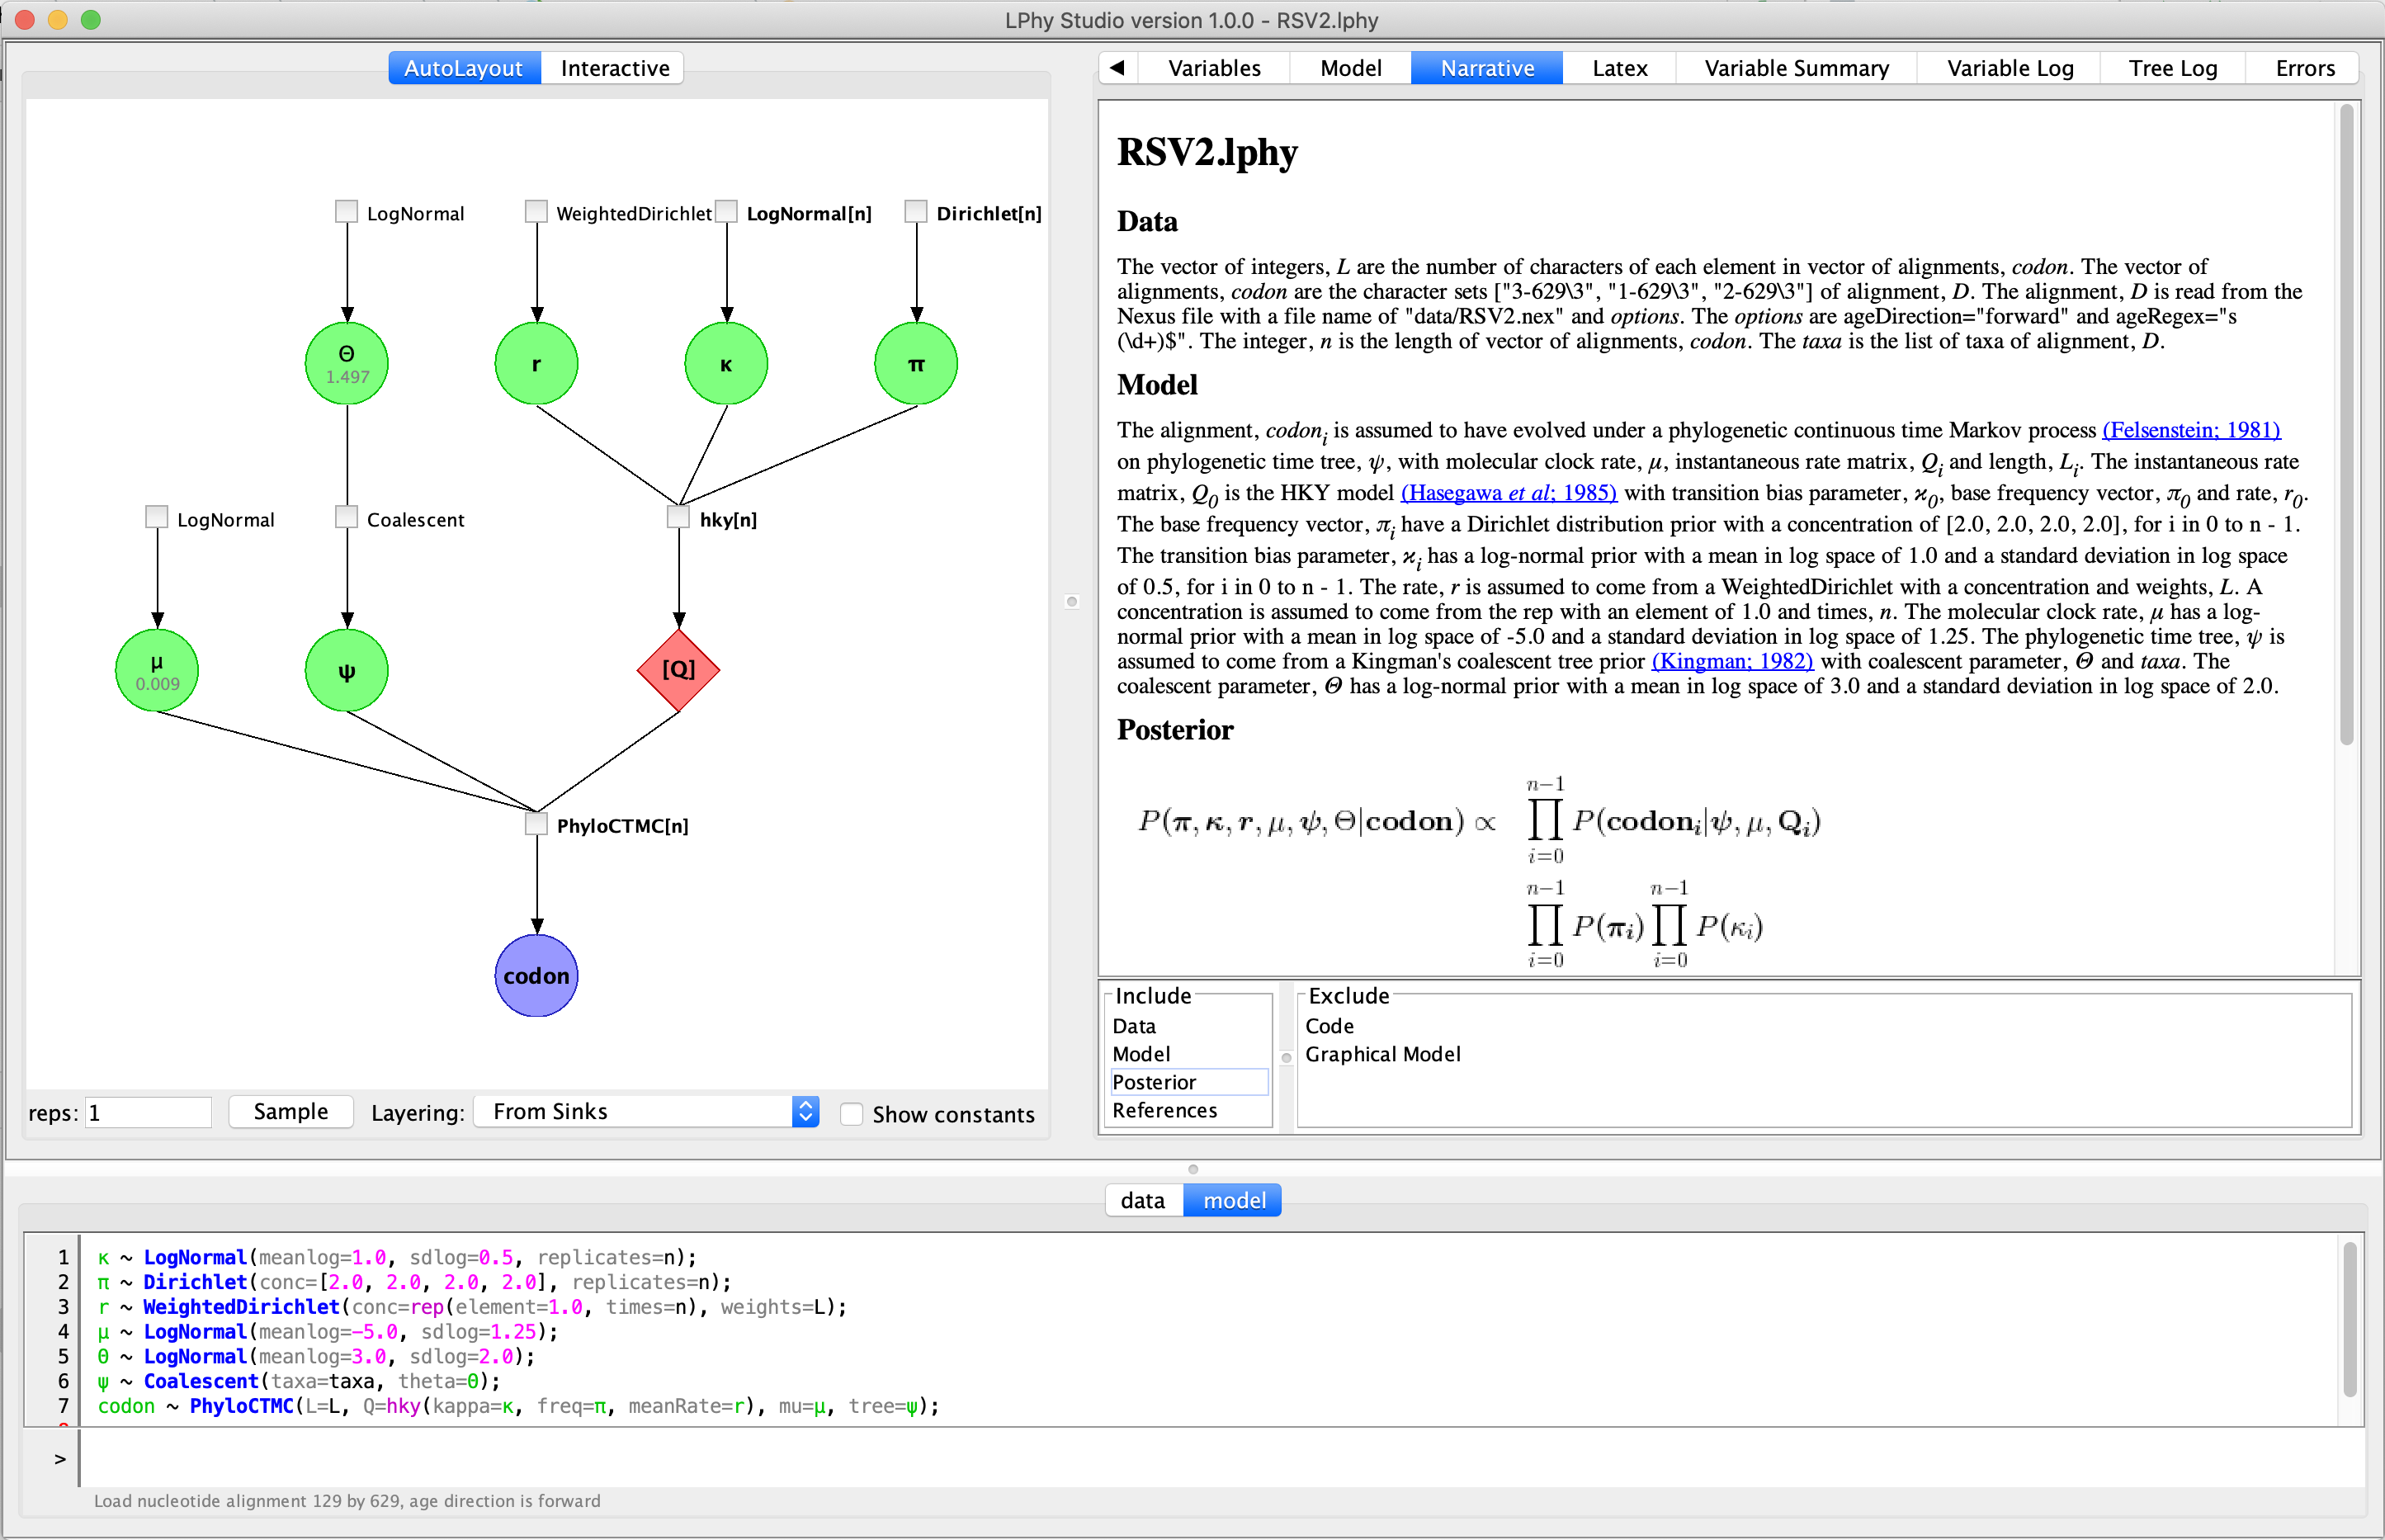
\includegraphics[width=\textwidth]{lphystudio_screenshot.png}
  \caption{A screenshot of LPhy Studio showing the probabilistic
    graphical model from Example \ref{lphy:rsva} on the left panel
    (constants are being hidden), and the automatically generated
    description of the data, the model and the posterior
    distribution on the right panel.} 
  \label{fig:lphystudio}
\end{figure}

\subsection*{Integration with phylogenetic analysis software BEAST2}
LPhyBEAST is a command-line program that takes an LPhy model
specification, and some data and produces a BEAST 2 XML input file.
It is therefore an alternative way to succinctly express and
communicate BEAST analyses.

\begin{itemize}
\item for evolutionary biologists
\begin{enumerate}
\item describe complex phylogenetic models succinctly and exactly
\item simulate prior distributions from these models, including arbitrary statistics
\item use model description to run inference on a real data set using LPhyBEAST
\item produce precise methods section and graphical model figure for describing analyses in published works
\end{enumerate}
\item for computational biologists
\begin{enumerate}
\item enable easy extension of the type system and generative distributions available using the extension mechanism of Lingua Phylo Studio (in Java programming language)
\item implement MCMC inference in BEAST2 for new models using LPhyBEAST and its extension mechanism
\item do well-calibrated simulation study that validate the implementation of inference framework
\end{enumerate}
\end{itemize}

\subsection*{Model validation}
...


\section*{Discussion}
...

\section*{Conclusion}
...

\section*{Supporting Information}

% Include only the SI item label in the paragraph heading. Use the \nameref{label} command to cite SI items in the text.
\paragraph*{S1 Fig.}
\label{S1_Fig}
{\bf Bold the title sentence.} Add descriptive text after the title of the item (optional).

\paragraph*{S2 Fig.}
\label{S2_Fig}
{\bf Lorem ipsum.} Maecenas convallis mauris sit amet sem ultrices gravida. Etiam eget sapien nibh. Sed ac ipsum eget enim egestas ullamcorper nec euismod ligula. Curabitur fringilla pulvinar lectus consectetur pellentesque.

\paragraph*{S1 File.}
\label{S1_File}
{\bf Lorem ipsum.}  Maecenas convallis mauris sit amet sem ultrices gravida. Etiam eget sapien nibh. Sed ac ipsum eget enim egestas ullamcorper nec euismod ligula. Curabitur fringilla pulvinar lectus consectetur pellentesque.

\paragraph*{S1 Video.}
\label{S1_Video}
{\bf Lorem ipsum.}  Maecenas convallis mauris sit amet sem ultrices gravida. Etiam eget sapien nibh. Sed ac ipsum eget enim egestas ullamcorper nec euismod ligula. Curabitur fringilla pulvinar lectus consectetur pellentesque.

\paragraph*{S1 Appendix.}
\label{S1_Appendix}
{\bf Lorem ipsum.} Maecenas convallis mauris sit amet sem ultrices gravida. Etiam eget sapien nibh. Sed ac ipsum eget enim egestas ullamcorper nec euismod ligula. Curabitur fringilla pulvinar lectus consectetur pellentesque.

\paragraph*{S1 Table.}
\label{S1_Table}
{\bf Lorem ipsum.} Maecenas convallis mauris sit amet sem ultrices gravida. Etiam eget sapien nibh. Sed ac ipsum eget enim egestas ullamcorper nec euismod ligula. Curabitur fringilla pulvinar lectus consectetur pellentesque.

\section*{Acknowledgments}
Thanks for the New Zealand eScience Infrastructure (NeSI) to provide the high performance computation resource for our model validations.

\nolinenumbers

% Either type in your references using
% \begin{thebibliography}{}
% \bibitem{}
% Text
% \end{thebibliography}
%
% or
%
% Compile your BiBTeX database using our plos2015.bst
% style file and paste the contents of your .bbl file
% here. See http://journals.plos.org/plosone/s/latex for 
% step-by-step instructions.
% 
\bibliography{linguaPhylo}



\end{document}

